\input ../preamble

\begin{document}

{\Huge

  \centerline{\bf TTIC 31230, Fundamentals of Deep Learning}
  \bigskip
  \centerline{David McAllester, Winter 2018}
  \vfill
  \centerline{\bf Invariant Theory}
  \vfill
  \vfill

\slide{Invariant Theory}

Why Are Early Filters Wavelets?

\centerline{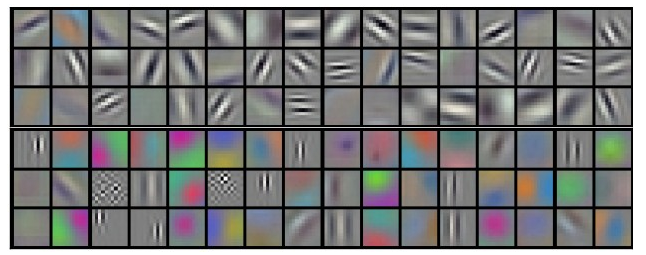
\includegraphics[width=5.0in]{../images/invariance} {\large Krizhevsky}}


\vfill
\centerline{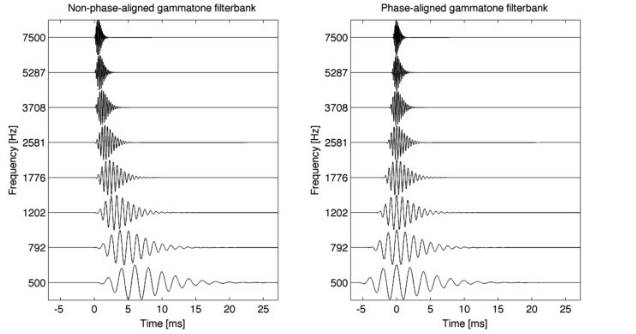
\includegraphics[width=5.0in]{../images/gammatones} {\large MathWorks}}
           
\slide{Invariance}
Consider the distribution of ``natural'' 360 degree images.

\vfill
It should be true that the probability of a given 360 degree image is equal to the probability of any rotation of that image.

\vfill
We say that the probability distribution is invariant to rotation.

\slide{Invariances}

Translation invariance (in both space and time)

\vfill
Scale invariance (in both space and time)

\vfill
Rotation invariance (spatial rotations).

\slide{PCA and Invariance}

\centerline{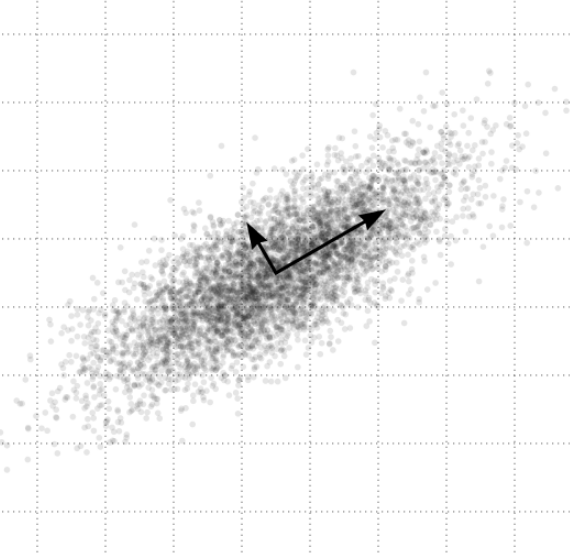
\includegraphics[height = 2in]{../images/PCA}}

\vfill
The principal components in PCA are the eigenvectors of the covariance matrix.

\vfill
The principal components of the covariance matrix of a translation invariant distribution are the Fourier basis functions
(sine and cosine).

\slide{PCA and Invariance}
The eigenvalues of the covariance matrix are given by the power spectrum of the signal distribution.

\vfill
This is the Einstein-Wiener-Khinchin theorem (proved by Wiener, and independently
by Khinchin, in the early 1930’s, but --- as only recently recognized —--
stated by Einstein in 1914). {\huge From ``Signals and Systems'' by Oppenheim and Verghese}

\vfill
This explains projection onto complex exponentials as a first step in signal processing and signal compression (e.g., JPEG).

\slide{More Formally}

Let $\rho$ be a probability density over vectors in $\reals^n$.

\vfill
We say $\rho$ is rotation-stationary if

\begin{itemize}
\item  $\expect{x_i} = \expect{x_j}$ for all $i,j$.

\item $\expect{x_ix_j} = f(i-j \bmod n)$
\end{itemize}

\vfill
Rotation stationarity is a simplification of the more widely used notion of translation stationarity (or just stationarity).

\slide{More Formally}

The covariance matrix is given by

\vfill
$$\Sigma_{i,j} = \expect{x_ix_j - \expect{x_i}\expect{x_j}} = g(i-j \bmod n)$$

\vfill
A matrix satisfying $\Sigma_{i,j} = g(i-j \bmod n)$ is called {\bf circulant}.

\vfill
The eigenvectors of a circulant matrix form a discrete 
Fourier basis.

\slide{Wavelets}

In practice we want the compressed representation to be local to also satisfy scale invariance.  This leads to {\bf wavelets}.

\vfill
To my knowledge scale invariance is not currently built into deep vision architectures.

\vfill
\centerline{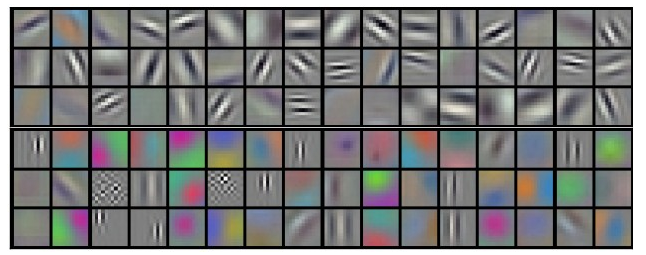
\includegraphics[width=7.0in]{../images/invariance}}

\slide{Invariance and Data Augmentation}

CNNs build translation invariance into the architecture.

\vfill
Another approach to invariance is to apply invariant transformations to the training data.

\vfill
For example we can apply translations, scalings, rotations, reflections to generate more labeled images in MNIST or Imagenet
to get a much larger training set.

\slide{END}
\end{document}
